%!TEX root = ../diploma.tex
\section{Постановка задачи}\label{sec:task}

Пусть $\mathbb{R}$ — множество вещественных чисел, будем называть
\textit{тензорами} многомерные массивы с элементами из $\mathbb{R}$, $\mathbb T
= \bigcup\limits_{n=1}^{\infty}\bigcup\limits_{\mathbb{T}_1,\ldots,\mathbb{T}_n
\in \left\{\mathbb{R}^{s} \mid s \in \mathbb{N}^{+}\right\}} \mathbb{T}_1 \times
\cdots \times \mathbb{T}_n$ — множество всевозможных кортежей из тензоров.

\Def{\emph{Ациклическим графом вычислений (АГВ)} назовем тройку $\langle G(V,
E), \mathbf{op}, \mathbf{t}\rangle$, где $G(V, E)$ — ориентированный
ациклический граф, в котором:
\begin{itemize}
    \item $\mathbf{op}: V \rightarrow (\mathbb T \rightarrow \mathbb T)$ —
    сопоставление вершинам операций, которые отображают набор входящих в вершину
    тензоров в набор выходящих.
    \item $\mathbf{t}: E \rightarrow \bigcup\limits_{s\in \mathbb{N}^{+}}
    \mathbb{R}^{s}$ — каждому ребру соответствует некоторый тензор, причем
    разные ребра могут соответствовать одному и тому же тензору тогда и только
    тогда, когда эти ребра исходят из одной вершины. \end{itemize}}

Вычисление предсказаний НС можно представить в виде АГВ, пример такого
представления приведен на Рис.~\ref{fig:cfg}. Данная работа сфокусирована на
улучшении программно-аппаратной части вычисления предсказаний НС, без
рассмотрения оптимизации архитектуры самой НС или процесса ее обучения. Целью
работы является исследование существующих методов оптимизации объема
используемой памяти и затраченного времени на вычисление предсказания НС на
уровне АГВ, а также разработка и реализация метода, позволяющего одновременно
оптимизировать и затраченное время, и объем используемой памяти.

\begin{figure}[h]
\centering
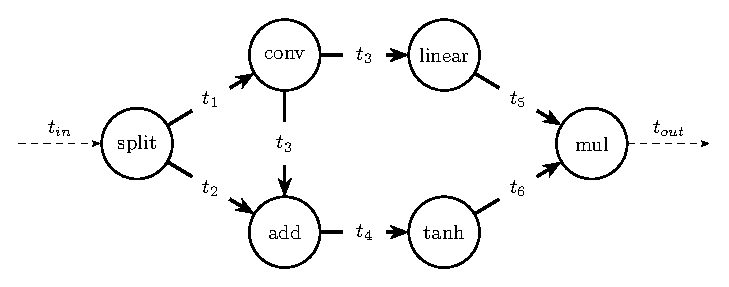
\includegraphics[scale=1.05]{dag.pdf}
\caption{Пример ациклического графа вычислений}
\label{fig:cfg}
Пунктирными линиями изображены входной и выходной тензор, которые присутствуют в
вычислениях, но отсутствуют в самом графе.
\end{figure}

\subsection{Задача оптимизации памяти}

Параметры НС, представляющие собой тензоры, можно разделить на четыре категории:
\begin{itemize}
    \item Константные, так же веса НС
    \item Входные — то, что подается на вход НС
    \item Выходные — предсказание НС
    \item Промежуточные — не относящиеся к трем остальным категориям
\end{itemize}
Входные и константные тензоры копируются из оперативной памяти в память ГП перед
вычислением сети, выходные — копируются из памяти ГП в оперативную память после
произведенных вычислений. Для промежуточных же тензоров память может быть
использована повторно, если это не нарушает корректности производимых
вычислений.

В настоящей работе мы рассматриваем задачу предварительного распределения
памяти, то есть размеры промежуточных тензоров НС заранее известны. Выделение
блока памяти производится указанием для промежуточных тензоров сдвигов на
соответствующие им ячейки памяти, начиная с которых тензоры могут быть записаны
или считаны, располагаясь как непрерывные блоки. Выбор такого подхода работы с
памятью обусловлен тем, что интерфейс прикладного программирования Vulkan,
используемый для реализации программно-аппаратной части MindSpore Lite,
предполагает резервирование приложением продолжительно используемой памяти,
которую он может самостоятельно использовать.

Для соблюдения корректности результата последовательное вычисление НС необходимо
производить в порядке любой топологической сортировки АГВ (ТС), т.е. для
вычисления в данный момент некоторой операции необходимо и достаточно, чтобы все
входные тензоры были вычислены.

\noindent\textbf{Формулировка задачи оптимального распределения памяти}

Обозначим множество тензоров, соответствующих ребрам в АГВ $\langle G(V, E),
\mathbf{op}, \mathbf{t}\rangle$, как ${T} = \text{im}(\mathbf{t}) =
\left\{\mathbf{t}(e_1), \ldots, \mathbf{t}(e_{|E|})\right\}$. Для тензора
$t\in{T}$ обозначим размер тензора, который он занимает в памяти, как
$w_t\in\mathbb{N}$. Тогда задачу распределения памяти можно задать в виде
следующей задачи оптимизации:
\begin{subequations}\label{eqn:opt}
    \renewcommand{\theequation}{\theparentequation\asbuk{equation}}
\begin{align}[left ={\empheqlbrace}]
    & \max\limits_{t\in {T}}(x_t+w_t) \rightarrow \min & \label{minmax} \\
    & x_{t_1} + w_{t_1} \le x_{t_2} \vee x_{t_2} + w_{t_2} \le x_{t_1} & \notag
    \\
    & \text{\ }\forall t_1,t_2 \in{T}: \text{$t_1$ и $t_2$ могут использоваться
    одновременно} & \label{cond:intersect} \\
    & x_t \in \mathbb{Z},\,x_t \ge 0 & \forall t\in {T} \label{cond:nonneg}
    \end{align}
\end{subequations}
где $x_t$ — сдвиг в памяти ячейки начала размещения тензора $t$.
Ограничение~\ref{cond:intersect} запрещает тензорам использовать одну и ту же
память, если может возникнуть конфликт, а~\ref{cond:nonneg} отражает то, что
сдвиг в памяти обязан быть целым неотрицательным числом. При этих ограничениях
требуется использовать как можно меньший объем памяти, этому соответствует
выражение~\ref{minmax}.

\subsection{Задача параллельных вычислений}

Вычисление НС с помощью программы представляется в виде конвейера из команд,
которые можно логически разбить на следующие типы:
\begin{enumerate}
    \item Копирование блока из оперативной памяти в память ГП\label{op:copyto}
    \item Копирование блока из памяти ГП в оперативную память\label{op:copyfrom}
    \item Исполнение вычислительного \textit{шейдера} (программы, выполняющейся
    параллельно несколькими блоками потоков ГП)\label{op:shaders}
    \item Барьер памяти вида запись/чтение между операциями типа~\ref{op:copyto}
    и операциями типа ~\ref{op:shaders}.\label{op:bar-copy-comp}
    \item Барьер памяти вида запись/чтение между операциями
    типа~\ref{op:shaders}  и операциями типа
    ~\ref{op:shaders}.\label{op:bar-comp-comp}
    \item Барьер памяти вида запись/чтение между операциями
    типа~\ref{op:shaders}  и операциями типа
    ~\ref{op:copyfrom}.\label{op:bar-comp-copy}
\end{enumerate}

Перед началом интересующих нас вычислений выполняются команды
типов~\ref{op:copyto} и~\ref{op:bar-copy-comp}, после —~\ref{op:bar-comp-copy}
и~\ref{op:copyfrom}. Операции (вершины в АГВ) суть один или несколько
вычислительных шейдеров, их вычисление относится к типу команд~\ref{op:shaders},
а между вычислением вершин размещаются при необходимости барьеры
памяти~\ref{op:bar-comp-comp}.

Под \textit{базовой программной реализацией} вычислений НС с помощью ГП будем
подразумевать следующее: вычисление операций происходит в порядке произвольной
топологической сортировки АГВ; между каждой последовательной парой операций в
конвейере располагается барьер памяти; для каждого тензора выделяется отдельный
блок памяти, непересекающийся ни в какой момент времени с остальными.

\begin{figure}
\centering
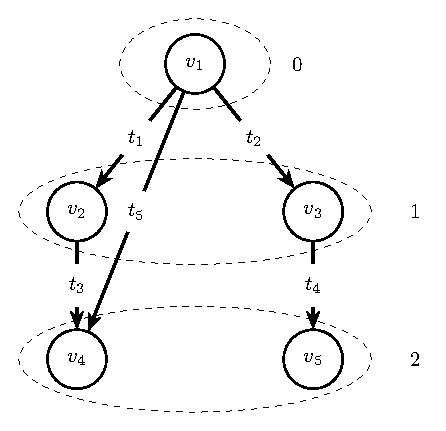
\includegraphics[scale=1.2]{par.pdf}
\caption{Пример АГВ, в котором возможно параллельное вычисление некоторых вершин}
\label{parcfg}
Пунктирными линиями обведены подмножества\\ независящих друг от друга вершин
\end{figure}

При такой реализации возникает проблема избыточных синхронизаций, вызывающих
простои в вычислениях. Сократить время простоев возможно, разбив АГВ на
несколько блоков так, что внутри каждого блока вершины будут попарно
\textit{независимы} (не существует пути из одной в другую), и можно выбрать
порядок вычисления этих блоков, при котором все зависимости будут соблюдаться
(аналогично топологической сортировке вершин). Пример такого разбиения приведен
на Рис.~\ref{parcfg}.

Задача параллельных вычислений состоит в том, чтобы найти эффективный способ
получать разбиение АГВ на непересекающиеся подмножества попарно независимых
вершин так, чтобы не было циклической зависимости этих подмножеств друг от
друга. Также нужно исследовать применимость способа на практике.
